\documentclass[answers]{exam}

\usepackage[spanish]{babel}
\usepackage{graphicx}

\newcommand{\materia}{Organización y Aquitectura de Computadoras}
\newcommand{\tarea}{Tarea 1}

\title{
  \huge \materia{} \\[0.5cm]
  \LARGE \tarea{}
}

\author{
  Nombre: José Ethan Ortega González \\
  Número de cuenta: 316088327
}

\renewcommand{\solutiontitle}{\noindent\textbf{Solución:}\par\noindent}
\runningheadrule{}
\runningheader{\materia{}}{\tarea{}}{\date{\today}}
\footer{}{Página \thepage\ de \numpages}{}

\begin{document}
\maketitle{}
\thispagestyle{headandfoot}
\begin{questions}
  \question{De la siguiente lista de lenguajes de programación indique si el
    lenguaje es de bajo nivel, medio nivel o alto nivel.
    \begin{center}
      \begin{tabular}{lllll}
        AT\&T  & Objective-C & PL/I          & Prolog              & Scheme \\
        Kotlin & C\#         & Natural       & Macro Assembler/370 & Fortran \\
        Erlang & Cobol       & SQL           & Scala               & MSDOS \\
        Elixir & Algol 8     & Assembly x86  & Modula              & GNU/GAS
      \end{tabular}
    \end{center}}
  \begin{solution}
    Organicé los lenguajes en una tabla:
    \begin{center}
      \begin{tabular}{|c|c|c|}
        \hline
        Bajo nivel          & Medio nivel & Alto nivel \\
        \hline
        Assembly x86        & Objective-C & Fortran \\
        PL/I                & C\#         & Algol 8 \\
        Macro Assembler/370 & Fortran     & Kotlin \\
        GNU/GAS             & PL/I        & SQL \\
                            & Scheme      & Natural \\
                            &             & Scala \\
                            &             & Prolog \\
                            &             & Modula \\
                            &             & Erlan \\
                            &             & Elixir \\
                            &             & Cobol \\
        \hline
      \end{tabular}
    \end{center}
    Hay unos ``impostores'' en la lista. AT\&T es una compañía que se enfoca en
    telefonía móvil, banda ancha, telefonía fija, seguridad del hogar, seguridad
    de red y servicios comerciales. Mientras que MSDOS fue el principal sistema
    operativo para computadoras personales compatible con IBM PC en la década de
    1980 y mediados de años 1990.
  \end{solution}

  \question{Menciona las cuatro unidades funcionales principales de una
    computadora y describe su funcionamiento.}
  \begin{solution}
    Las cuatro unidades funcionales principales de una computadora son:
    \begin{itemize}
      \item \textbf{Memoria:} Se utiliza como memoria de trabajo de computadoras
            y otros dispositivos para el sistema operativo, los programas y la
            mayor parte del software.
      \item \textbf{Unidad Central de Proceso:} Su trabajo es interpretar las
            instrucciones de un programa informático mediante la realización de
            las operaciones básicas aritméticas, lógicas y externas
            (provenientes de la unidad de entrada/salida). Su diseño y avance ha
            variado notablemente desde su creación, aumentando su eficiencia y
            potencia, y reduciendo aspectos como el consumo de energía y el
            costo.
            \begin{itemize}
              \item \textbf{Unidad de Control:} Su función es buscar las
                    instrucciones en la memoria principal, decodificarlas
                    (interpretación) y ejecutarlas, empleando para ello la
                    unidad de proceso.
              \item \textbf{Unidad Aritmético-Lógica:} Es un circuito digital
                    que realiza operaciones aritméticas (suma, resta) y
                    operaciones lógicas (AND, OR, NOT) entre los valores de los
                    argumentos.
            \end{itemize}
      \item \textbf{Dispositivos de entrada:} Son todos aquellos dispositivos
            que permiten introducir datos o información en una computadora para
            que esta los procese u ordene.
      \item \textbf{Dispositivos de salida:} Son todos aquellos dispositivos que
            permiten transformar la información del CPU en un formato que sea
            entendible para los humanos.
    \end{itemize}
  \end{solution}

  \question{¿Qué ventajas y desventajas puedes encontrar en el modelo de la
    arquitectura de Von Neumann? Argumenta tu respuesta.}
  \begin{solution}
    La principal desventaja es que la memoria RAM que es donde se encuentran las
    instrucciones y los datos que han de ser procesados se encuentran unificados
    y compartidos a través un mismo bus de datos y direccionamiento común. Por
    lo que las instrucciones y los datos han de ser captados de manera
    secuencial desde la memoria.
  \end{solution}

  \question{La Arquitectura Von Neuman fue descrita por el matemático y físico
    John von Neumann y otros, en el primer borrador de un informe sobre el
    EDVAC. Pero la computación de 1945 a la actualidad ha dado pasos
    agigantados, aumentando la complejidad de la arquitectura inicial, la base
    de su funcionamiento es la misma. ¿Qué cambios aprecias hoy en día en tu
    computador que no se ven descritos por el diagrama dado en 1945? Argumenta
    tu respuesta.}
  \begin{solution}
    El cambio más notorio es que, en la actualidad, nos hemos pasado a los
    procesadores multinúcleo. Un procesador multinúcleo es aquel que combina dos
    o más microprocesadores independientes en un solo paquete, a menudo un solo
    circuito integrado. Un dispositivo de doble núcleo contiene solamente dos
    microprocesadores independientes. En general, los microprocesadores
    multinúcleo permiten que un dispositivo computacional exhiba una cierta
    forma del paralelismo a nivel de thread sin incluir múltiples
    microprocesadores en paquetes físicos separados.
  \end{solution}

  \newpage{}

  \question{En la siguiente imagen, se nos muestra la disyunción y la conjunción
    proposicional usando interruptores. Usando ese mismo modelo, ¿cómo sería un
    XOR usando interruptores?
    \begin{figure}[h!]
      \centering
      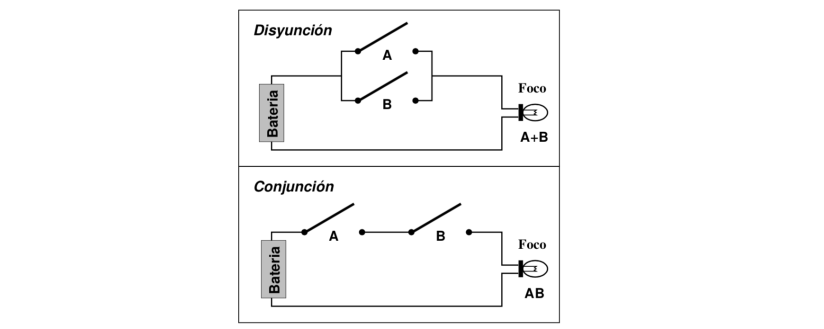
\includegraphics[width=\textwidth]{2021-10-14_22-59}
    \end{figure}

    Escanea tu respuesta, usa un software que te ayude a modelarlo o usa alguna
    de las paqueterías de \LaTeX{} para modelar tu respuesta.}
  \begin{solution}
    El circuito es el siguiente:
    \begin{center}
      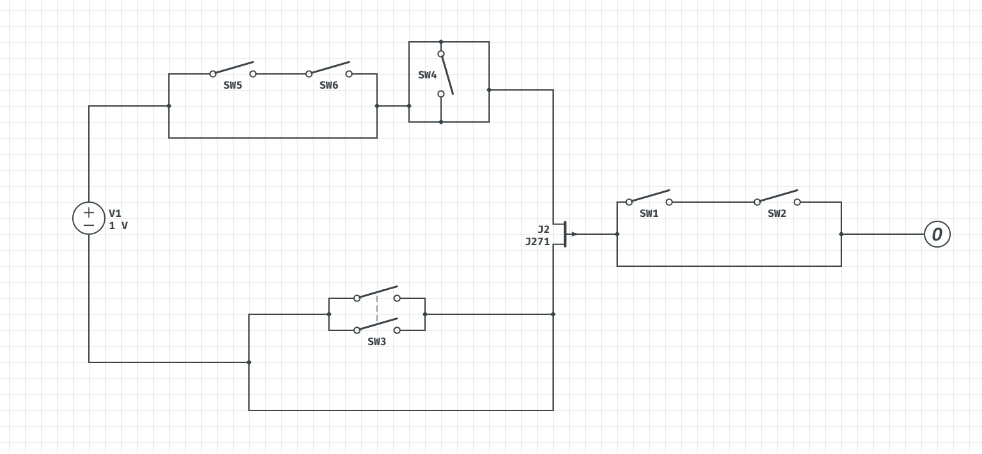
\includegraphics[width=\textwidth]{2021-10-14_23-39}
    \end{center}
  \end{solution}
\end{questions}
\end{document}
